\documentclass[12pt,a4paper,utf8]{ctexart}
\usepackage{ctex,amsmath,amssymb,subfig,cite,graphicx,diagbox,fontspec,fancyhdr,geometry}
\usepackage[ntheorem]{empheq}
\usepackage{enumitem,fullpage,cleveref,cellspace,listings,color,framed}
\definecolor{gray}{rgb}{0.5,0.5,0.5}
\definecolor{dkgreen}{rgb}{.068,.578,.068}
\definecolor{dkpurple}{rgb}{.320,.064,.680}

%set Fortran styles
\lstset{
    frameround=tftf,
    language=Fortran,
    keywords={SELECT,PROGRAM,PRINT,STOP,END,WRITE,INTEGER,REAL,COMPLEX,CHARACTER,LOGICAL,READ,FORMAT,IMPLICIT,PARAMETER,DATA,EQUIVALENCE,TYPE,PAUSE,CONTINUE,CYCLE,EXIT,IF,SELECT,DO,ALLOCATE,DEALLOCATE,WHERE,FORALL,SUBROUTIHNE,CALL,RETURN,FUNCTION,COMMON,BLOCK DATA,SAVE,INTERFACE,CONTAIN,MODULE,USE,PUBLIC,PRIVATE,ENTRY,OPEN,INQUIRE,CLOSE,NAMELIST,POINTER,NULLFY,REWIND,BACKSPACE,ENDFILE
    },
    basicstyle=\small\ttfamily,
    numbers=left,
    numberstyle=\small,
    keywordstyle=\color{blue}\bfseries,
    commentstyle=\color{dkgreen},
    stringstyle=\color{dkpurple},
    backgroundcolor=\color{white},
    tabsize=2,
    showspaces=false,
    showstringspaces=false,
    breaklines=true,
    frame=trBL,
}
\CTEXsetup[format+={\raggedright}]{section}
\setlength{\parindent}{2em}
\geometry{
    textwidth=138mm,
    textheight=215mm,
    left=27mm,
    right=27mm,
    top=25.4mm,
    bottom=25.4mm,
    headheight=2.17cm,
    headsep=4mm,
    footskip=12mm,
    heightrounded,
}
\pagestyle{fancy}
\lhead{\textsl{2021秋-计算物理A}}
\chead{}
\rhead{\textsl{PB19020634-于浩然}}
\lfoot{}
\cfoot{\thepage}
\rfoot{}

\begin{document}
\begin{center}
    {\LARGE\textbf{计算物理作业七}}\\
    \textrm{于浩然}~~~~~~\textrm{PB19020634}~~~~~~\textrm{2021.10.20}
\end{center}

\section{作业题目}

对一个实验谱数值曲线
$p(x)$,自设$F(x)$,分别用直接抽样法和舍选法对$p(x)$抽样.比较原曲线和抽样得到的曲线以验证.讨论其抽样效率.

\begin{figure}[htp]
    \centering
    \includegraphics[width=0.8\textwidth]{tit.png}
    \caption{实验谱数值曲线$p(x)$示意图}
    \end{figure}

\section{算法简介}

\subsection{离散点的直接抽样法}

设变量$x$是离散型的,取值为$x_1,
x_2,\cdots$,相应值出现的概率为$p_1,p_2,\cdots$.
如果从$[0,1]$区间中均匀抽样得到的随机数满足下式:
\begin{equation}
    \sum_{i=1}^{n-1} p_i < \xi < \sum_{i=1}^{n} p_i
\end{equation}
则物理量$x$取值为$x_n$.

\subsection{舍选抽样法}

考虑到所给数据是一简单分布,为简单期间我们直接考虑用分段阶梯函数作为比较函数的舍选法.
根据 \texttt{DATA.txt}文件所给数据,不妨取$M_1 = 5700$,$M_2 =
38000$,比较函数为如下形式:
\begin{equation}
    F(x) = 
    \begin{cases}
        M_1,\quad 2900 \leq x \leq 2990 \\
        M_2,\quad 2990 \leq x \leq 3014
    \end{cases}
\end{equation}

根据舍选法的一般形式:
\begin{enumerate}
    \item[(1)] 产生一对$[0,1]$上均匀分布的随机抽样值$(\xi_1,
        \xi_2)$,抽样表示式为:
        \begin{equation}
            \xi_1 = \int _{2900} ^{\xi_x} F(x) \textrm{d}x \big/ \int _{2900}
            ^{3014} F(x)
            \textrm{d}x,\quad \xi_y = \xi_2 F(\xi_x) 	 	
        \end{equation}
        即:
        \begin{equation}
            \xi_1 = 
            \begin{cases}
                \frac{(\xi_x - 2900)M_1}{90M_1 + 24M_2},\quad 2900 \leq \xi_x \leq 2990
                \\
                \frac{90M_1 + (\xi_x - 2990)M_2}{90M_1 + 24M_2},\quad 2990 \leq
                \xi_x \leq 3014
            \end{cases}
        \end{equation}
        \begin{equation}
            \xi_2 =
            \begin{cases}
                \xi_y / M_1,\quad 2900 \leq \xi_x \leq 2990 \\
                \xi_y / M_2,\quad 2990 \leq \xi_x \leq 3013
            \end{cases}
        \end{equation}
    \item[(2)]判断条件$\xi_y \leq p(\xi_x)$是否成立:
        \begin{itemize}
            \item $2900 \leq \xi_x \leq 2990$
            \begin{equation}
                \xi_x = 2900 + (90 + 24M_2/M_1)\xi_1 \leq 2990 \Rightarrow 0
                \leq \xi_1
                \leq \frac{90}{90 + 24M_2/M_1}
            \end{equation}
            
            判断条件为
            \begin{equation}
                M_1 \xi_2 \leq p(2900 + (90 + 24M_2/M_1)\xi_1)
            \end{equation}
            时,取$\xi_x$.

            \item $2990 \leq \xi_x \leq 3013$
            \begin{equation}
                \xi_x = 2990 + (90M_1/M_2 + 24)\xi_1 - 90M_1/M_2
                \Rightarrow\frac{90}{90 + 24M_2/M_1} \leq \xi_x \leq 1
            \end{equation}

            判断条件为
            \begin{equation}
                M_2 \xi_2 \leq 
            p(2900 + (90M_1/M_2 + 24)\xi_1 - 90M_1/M_2)
            \end{equation}
            时,取$\xi_x$.
        \end{itemize}
        若判断条件不成立,则舍.
    \end{enumerate}
\section{编程实现}

用FORTRAN90进行程序编写,分别展示如下.

\subsection{离散点的直接抽样法}

按照我们在2.1中所简述的方法,用一个子程序实现这一过程,将代码展示如下.由于所给实验
谱数据为一个$2\times 114$的二维数组,在这里我们用一个长度为228的一维数组
\texttt{dat}来存放这些数据,其中奇数项为$energy(eV)$值,偶数项为$Intensity$值.
\begin{framed}
\begin{lstlisting}[language=Fortran]
SUBROUTINE DscSample(p) !离散(discrete)直接抽样
    INTEGER(KIND=4) :: p, i, j
    INTEGER(KIND=8) :: S = 0, dat(228) !奇数项dat(2i-1)为x值,偶数项dat(2i)为y值
    REAL(KIND=8) :: sumprob(114) !几率求和值
    REAL(KIND=8), DIMENSION(10**p) :: xi, x
    OPEN (1, file='xi_1.dat') !从其中一个文件导入10^5个[0,1]上均匀分布的随机数
    READ (1, *) xi
    CLOSE (1)
    OPEN (1, file='data.TXT') !读取实验谱数据
    READ (1, *) dat
    CLOSE (1)
    DO i = 1, 114
        S = S + dat(2 * i) !求粒子总数
    END DO
    sumprob(1) = real(dat(2)) / S !使用real()函数转换为实型使除法有意义
    DO i = 2, 114
        sumprob(i) = sumprob(i - 1) + real(dat(2 * i)) / S
    END DO
    DO i = 1, 10**p
        DO j = 1, 114 
            IF(xi(i) < sumprob(j)) THEN
                x(i) = dat(2 * j - 1) !将x轴值作为抽出的数据
                EXIT
            END IF
        END DO
    END DO
    OPEN (1, file='dscsmp.dat') !将抽出数组x写入文件
    WRITE (1, *) x
    CLOSE (1)
END SUBROUTINE DscSample
\end{lstlisting}
\end{framed}

另外为了将数据可视化与原曲线比较,用python脚本绘制直方图,代码如下:

\begin{framed}
\begin{lstlisting}[language=python]
import numpy as np
import matplotlib.pyplot as plt
import math

plt.rcParams['savefig.dpi'] = 300
plt.rcParams['figure.dpi'] = 300

data = np.loadtxt('dscsmp.dat')
plt.xlabel('energy(eV)')
plt.ylabel('Intensity(counts)')
plt.hist(data, bins=114)
plt.savefig('fig_2.eps')
\end{lstlisting}
\end{framed}

\subsection{舍选抽样法}
    将舍选法所用数据$M_1 = 5700,M_2 = 38000$代入参数,可得:
    \begin{equation}
        \frac{90}{90 + 24M_2/M_1} = 0.360000 \equiv C
    \end{equation}
    
    本FORTRAN90程序直接使用Schrage方法产生的一对$10^5$个随机数序列,
    分别使用种子461655342和96145235,附于附件中.

    由于 \texttt{data.TXT}
    所给的数据为离散数据,故我们在进行比较时使用
    \texttt{int()}函数将由均匀随机数序列生成的$[2900,3014]$中的浮点型随机数
    \textbf{转化为整型},
    再与 \texttt{intensity}
    中的实验谱数据进行比较(如20行、25行).在后面的计算结果中将讨论这种做法的可行性.

\begin{framed}
\begin{lstlisting}[language=Fortran]
SUBROUTINE Sample(p) !舍选法抽样
    INTEGER(KIND=4) :: dat(228), intensity(114), p , i
    REAL(KIND=8) ,PARAMETER :: C = 0.36 !定义的常数C,是xi_1的分界线
    REAL(KIND=8) ,DIMENSION(10**p) :: xi_1, xi_2, xi_x, x
    OPEN (1, file='data.TXT')
    READ (1, *) dat
    CLOSE (1)
    DO i = 1, 114
        intensity(i) = dat(2 * i) !将data中的y值写入数组,索引i对应energy为(2899+i)eV
    END DO
    OPEN (1, file='xi_1.dat') !将均匀分布的两个随机数序列写入数组xi_1, xi_2
    READ (1, *) xi_1
    CLOSE (1)
    OPEN (1, file='xi_2.dat')
    READ (1, *) xi_2
    CLOSE (1)
    DO i = 1, 10**p
        IF (xi_1(i) < C) THEN
            xi_x(i) = 2900 + (90 + 24 * 38000.0 / 5700) * xi_1(i)
            IF (5700 * xi_2(i) <= intensity(int(xi_x(i)) - 2899)) THEN
                x(i) = xi_x(i) !若上面的判断条件满足则取xi_x(i)作为抽样结果x(i)
            END IF
        ELSE
            xi_x(i) = 2990 + (90 * 5700.0 / 38000 + 24) * xi_1(i) - 90 * 5700.0 / 38000
            IF (38000 * xi_2(i) <= intensity(int(xi_x(i)) - 2899)) THEN
                x(i) = xi_x(i)
            END IF
        END IF
    END DO
    OPEN (1, file='smp.dat')
    DO i = 1, 10**p
        IF(x(i) .ne. 0) THEN
            WRITE (1,*) x(i) !将非零值(成功抽出的值)写入文件
        END IF
    END DO
    CLOSE (1)
END SUBROUTINE Sample       
\end{lstlisting}
\end{framed}

用python绘制直方图,代码如下:
\begin{framed}
\begin{lstlisting}[language=python]
import numpy as np
import matplotlib.pyplot as plt
import math

plt.rcParams['savefig.dpi'] = 300
plt.rcParams['figure.dpi'] = 300

data = np.loadtxt('data.TXT')
plt.xlabel('energy(eV)')
plt.ylabel('Intensity(counts)')
plt.hist(ex, bins=114)
plt.savefig('fig_1.eps')
\end{lstlisting}
\end{framed}

\section{计算结果}

\subsection{直接抽样法}

直方图显示如下:
\begin{figure}[htpb]
    \centering
    \includegraphics[width=0.8\textwidth]{fig_2.eps}
    \caption{直接抽样法结果直方图}
\end{figure}

图中纵轴为取值为特定整型值的抽样点的个数.可见,直接抽样法很好地显示了原曲线的特征,
对于这种取值点数较少的离散型抽样有很好的可行性.
\subsection{舍选抽样法}
将绘制的直方图显示如下:
\begin{figure}[htpb]
    \centering
    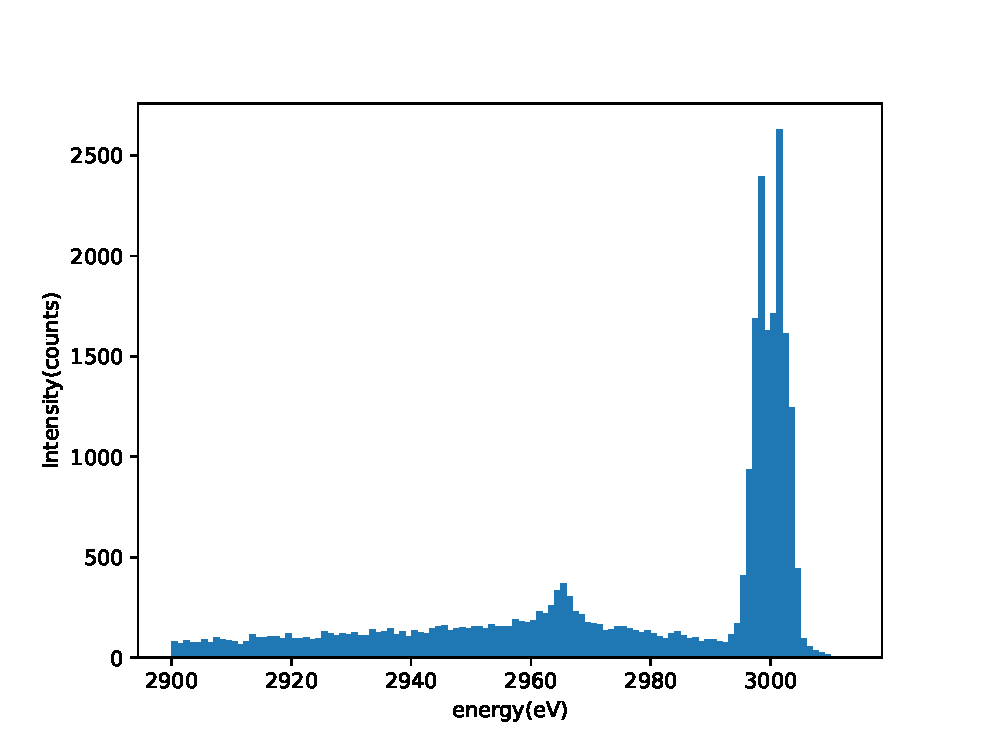
\includegraphics[width=0.8\textwidth]{fig_1.eps}
    \caption{舍选抽样法结果直方图}
\end{figure}

从此直方图可以明显看出实验谱数值曲线的轮廓,在$2665eV$的峰十分明显,在$3001eV$的峰也有明显的
轮廓,但在峰中心的值偏少,然而在直接抽样法的结果中也出现了这一情况,表明这应是所给数据
性质所导致的.舍选抽样法也得到了很好的结果.

从此数据实验的结果来看,我们对此离散数据谱的连续化是合理的.

考虑抽样效率,10000个随机点结果抽出27720个点,可得抽样效率:
\begin{equation}
    \frac{27720}{100000} = 0.2772
\end{equation}
\section{结论}
本题运用两种抽样法都得到了很好的模拟结果,我们加深了对舍选抽样的理解,并熟练了离散化数据
直接抽样的步骤.
\end{document}
